% ---------------- PAGE 1 ----------------
\setcounter{page}{1}

% Header: Logo left, Name right
%\noindent
%\begin{minipage}[t]{0.5\textwidth}
%\includegraphics[height=14mm]{logo.jpeg} % change if your file is logo.png
%\end{minipage}
%\begin{minipage}[t]{0.5\textwidth}
%\raggedleft
%{\Large\textbf{Keerthi M}}
%\end{minipage}

%\vspace{6mm}

% Series / Set
\noindent\fbox{\large Series ONS}\hfill\fbox{\large SET-1}

\vspace{6mm}

% Code No (Hindi + English)
\noindent\hfill
{\hindi कोड नं.}\quad \textbf{Code No. \Large 65/1/C}

\vspace{6mm}

% Roll No boxes (approx)
\noindent
\begin{minipage}[t]{0.55\textwidth}
{\hindi रोल नं.}\\
\textbf{Roll No.}\hspace{6mm}
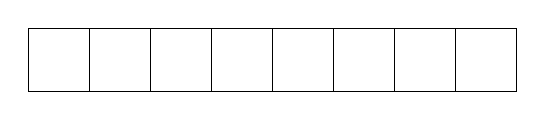
\begin{tikzpicture}[baseline]
\draw (0,0) rectangle (6.2,0.8);
\foreach \x in {0.775,1.55,2.325,3.1,3.875,4.65,5.425} {
  \draw (\x,0) -- (\x,0.8);
}
\end{tikzpicture}
\end{minipage}
\begin{minipage}[t]{0.45\textwidth}
\fbox{\parbox{\linewidth}{%
\hindi परीक्षार्थी कोड को उत्तर-पुस्तिका के मुख-पृष्ठ पर अवश्य लिखें।\\
Candidates must write the Code on the title page of the answer-book.
}}
\end{minipage}

\vspace{8mm}

% Instructions box (PASTE OCR TEXT HERE and correct it)
% Instructions box
\noindent\fbox{%
  \parbox{\textwidth}{\small
    \begin{itemize}[leftmargin=*, itemsep=4pt]
      \item \textHindi{कृपया जाँच कर लें कि इस प्रश्न-पत्र में मुद्रित पृष्ठ 11 हैं।}
      \item \textHindi{प्रश्न-पत्र में दाहिनी ओर दिए गए कोड नम्बर को छात्र उत्तर-पुस्तिका के मुख-पृष्ठ पर लिखें।}
      \item \textHindi{कृपया जाँच कर लें कि इस प्रश्न-पत्र में 26 प्रश्न हैं।}
      \item \textHindi{कृपया प्रश्न का उत्तर लिखना शुरू करने से पहले, प्रश्न का क्रमांक अवश्य लिखें।}
      \item \textHindi{इस प्रश्न-पत्र को पढ़ने के लिए 15 मिनट का समय दिया गया है। प्रश्न-पत्र का वितरण पूर्वाह्न 10.15 बजे किया जाएगा। 10.15 बजे से 10.30 बजे तक छात्र केवल प्रश्न-पत्र को पढ़ेंगे और इस अवधि के दौरान वे उत्तर-पुस्तिका पर कोई उत्तर नहीं लिखेंगे।}
      \item Please check that this question paper contains 11 printed pages.
      \item Code number given on the right hand side of the question paper should be written on the title page of the answer-book by the candidate.
      \item Please check that this question paper contains 26 questions.
      \item \textbf{Please write down the Serial Number of the question before attempting it.}
      \item 15 minute time has been allotted to read this question paper.
    \end{itemize}
  }%
}
\vspace{10mm}

% Title
\begin{center}
{\hindi \Large गणित}\\[2mm]
{\LARGE \textbf{MATHEMATICS}}
\end{center}

\vspace{8mm}

% Time/Marks
\noindent
\begin{minipage}[t]{0.5\textwidth}
{\hindi निर्धारित समय : 3 घण्टे}\\
\textit{Time allowed : 3 hours}
\end{minipage}
\begin{minipage}[t]{0.5\textwidth}
\raggedleft
{\hindi अधिकतम अंक : 100}\\
\textit{Maximum Marks : 100}
\end{minipage}

\vfill

% Footer
\noindent
65/1/C\hfill 1\hfill \textbf{P.T.O.}